% Created 2021-06-03 jue 12:15
% Intended LaTeX compiler: pdflatex
\documentclass[presentation,aspectratio=169]{beamer}
\usepackage[utf8]{inputenc}
\usepackage[T1]{fontenc}
\usepackage{graphicx}
\usepackage{grffile}
\usepackage{longtable}
\usepackage{wrapfig}
\usepackage{rotating}
\usepackage[normalem]{ulem}
\usepackage{amsmath}
\usepackage{textcomp}
\usepackage{amssymb}
\usepackage{capt-of}
\usepackage{hyperref}
\usepackage{khpreamble}
\usepackage{amssymb}
\usepgfplotslibrary{groupplots}
\newcommand*{\shift}{\operatorname{q}}
\DeclareMathSymbol{\Omega}{\mathalpha}{letters}{"0A}% italics
\DeclareMathSymbol{\varOmega}{\mathalpha}{operators}{"0A}% upright
\providecommand*{\upOmega}{\varOmega}% for siunitx
\usepackage[binary-units=true]{siunitx}
\usepackage{circuitikz}
\usetikzlibrary{calc}
\usetheme{default}
\author{Kjartan Halvorsen}
\date{2021-06-03}
\title{Espacio de estados  - polos, función de transferencia}
\hypersetup{
 pdfauthor={Kjartan Halvorsen},
 pdftitle={Espacio de estados  - polos, función de transferencia},
 pdfkeywords={},
 pdfsubject={},
 pdfcreator={Emacs 26.3 (Org mode 9.4.4)}, 
 pdflang={English}}
\begin{document}

\maketitle

\section{Mass-spring-damper, acceleration as output}
\label{sec:org90cc8bb}
\begin{frame}[label={sec:orgbb1aca3}]{Masa-resorte-amortiguador}
\begin{center}
\includegraphics[width=0.2\linewidth]{../../figures/mass-spring-damper.png}
\end{center}

\(x = \begin{bmatrix} X & \dot{X} \end{bmatrix}\). La aceleración \(\ddot{X}\) como señal de salida.

\begin{center}
\Large
\begin{align*}
  \dot{x} &= \overbrace{\begin{bmatrix} \textcolor{red!80!black}{0} & \textcolor{red!80!black}{0}\\ \textcolor{red!80!black}{-\frac{k}{m}}  & \textcolor{red!80!black}{-\frac{c}{m}} \end{bmatrix}}^A x  + \overbrace{\begin{bmatrix} \textcolor{red!80!black}{0} \\ \textcolor{red!80!black}{\frac{1}{m}} \end{bmatrix}}^B  u \\
       y &=  \underbrace{\begin{bmatrix} \textcolor{white}{-\frac{k}{m}}  & \textcolor{white}{-\frac{c}{m}} \end{bmatrix}}_C x + \underbrace{\begin{bmatrix} \textcolor{white}{\frac{1}{m}} \end{bmatrix}}_D u
\end{align*}

\end{center}
\end{frame}


\begin{frame}[label={sec:orgbeb5907}]{Masa-resorte-amortiguador}
\begin{center}
\includegraphics[width=0.2\linewidth]{../../figures/mass-spring-damper.png}
\end{center}

\(x = \begin{bmatrix} X & \dot{X} \end{bmatrix}\). La aceleración \(\ddot{X}\) como señal de salida.

\begin{center}
\Large
\begin{align*}
  \dot{x} &= \overbrace{\begin{bmatrix} \textcolor{red!80!black}{0} & \textcolor{red!80!black}{0}\\ \textcolor{red!80!black}{-\frac{k}{m}}  & \textcolor{red!80!black}{-\frac{c}{m}} \end{bmatrix}}^A x  + \overbrace{\begin{bmatrix} \textcolor{red!80!black}{0} \\ \textcolor{red!80!black}{\frac{1}{m}} \end{bmatrix}}^B  u \\
       y &=  \underbrace{\begin{bmatrix} \textcolor{red!80!black}{-\frac{k}{m}}  & \textcolor{red!80!black}{-\frac{c}{m}} \end{bmatrix}}_C x + \underbrace{\begin{bmatrix} \textcolor{red!80!black}{\frac{1}{m}} \end{bmatrix}}_D u
\end{align*}

\end{center}
\end{frame}


\section{Canonical forms}
\label{sec:org39f0f45}

\begin{frame}[label={sec:org7ff4df3}]{Formas canonicas}
\begin{itemize}
\item Forma controlable
\item Forma observable
\end{itemize}

\begin{block}{Recurso}
\href{https://lpsa.swarthmore.edu/Representations/SysRepTransformations/TF2SS.html}{https://lpsa.swarthmore.edu/Representations/SysRepTransformations/TF2SS.html}
\end{block}
\end{frame}

\section{Estabilidad}
\label{sec:orga469b44}

\begin{frame}[label={sec:org4dcda55}]{Estabilidad}
La solución homógena de \(\dot{x} = Ax\)  se puede escribir
\[ x(t) = \mathrm{e}^{\lambda_1 t}\alpha_1v_1 + \mathrm{e}^{\lambda_2 t}\alpha_2v_2 + \cdots + \mathrm{e}^{\lambda_n t}\alpha_nv_n,\]
donde \(\lambda_1\), \(\lambda_2\), \(\ldots\), \(\lambda_n\) son los \alert{eigenvalores} de \(A\). 

Estabilidad requiere que \alert{cada una} de las funciones exponenciales va hacia cero.
\[\Rightarrow \qquad \mathrm{Re}\{\lambda_i\} < 0, \; \forall i=1,2,3\ldots, n\]

Los eigenvalores de \(A\) son los \alert{polos} del sistema.
\end{frame}

\begin{frame}[label={sec:orgcfd4fee}]{Los eigenvalores}
\(\lambda\) y \(v\) es un par de eigenvalor y eigenvector de la matriz \(A\) si
\[Av = \lambda v\]
\pause
\[ \lambda v - Av = 0\]
\pause
\[ (\lambda I - A)v = 0\]
\pause
Para que la ecuación tenga soluciones no-triviales
 \[ \det (\lambda I - A) = 0 \quad \leftarrow \text{\alert{Ecuación característica}}\]
\end{frame}


\section{Modelo compartamental}
\label{sec:org52d7782}

\begin{frame}[label={sec:org11e4423}]{De espacio de estados a función de transferencia}
\end{frame}

\begin{frame}[label={sec:org92c1e04}]{Modelo compartimental}
 \small
\begin{columns}
  \begin{column}{0.5\linewidth}
    \begin{center}
      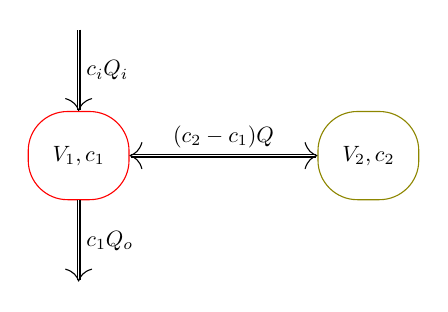
\begin{tikzpicture}[scale=0.8, transform shape,
	compartment/.style={rounded corners=5mm, minimum height=14mm, minimum width=16mm},
	node distance=46mm,
	]

	\node[compartment, draw=red, ] (comp1) {$V_1, c_1$};
	\node[compartment, right of=comp1, draw=olive,] (comp2) {$V_2, c_2$};

	\node[coordinate, above of=comp1, node distance=20mm] (input) {};
	\node[coordinate, below of=comp1, node distance=20mm] (output) {};

	\draw[->, double] (input) -- node[right]{$c_{i}Q_i$} (comp1);
	\draw[->, double] (comp1) -- node[right]{$c_{1}Q_o$} (output);
	\draw[<->, double] (comp1) -- node[above]{$(c_{2}-c_1)Q$} (comp2);

      \end{tikzpicture}
    \end{center}

  \end{column}
  \begin{column}{0.5\linewidth}
    \begin{equation*}
      \begin{aligned}
	V_1\frac{dc_1}{dt} &= Q(c_2-c_1) - Q_{o}c_1 + Q_ic_{i}, \quad  & c_1 \geq 0 \\
	V_2\frac{dc_2}{dt} &= Q(c_1-c_2),  & c_2 \geq 0,
      \end{aligned}
    \end{equation*}
  \end{column}
\end{columns}

\begin{center}
\Large
\begin{align*}
  \dot{x} &= \overbrace{\begin{bmatrix} \textcolor{red!80!black}{-\frac{Q+Q_o}{V_1}}  & \textcolor{red!80!black}{\frac{Q}{V_1}}\\
              \textcolor{red!80!black}{\frac{Q}{V_2}}  & \textcolor{red!80!black}{-\frac{Q}{V_2}}\end{bmatrix}}^A \begin{bmatrix} {x_1}\\ {x_2}\end{bmatrix}  + \overbrace{\begin{bmatrix} \textcolor{red!80!black}{\frac{1}{V_1}} \\ \textcolor{red!80!black}{0} \end{bmatrix}}^B  u \\
       y &=  \underbrace{\begin{bmatrix} \textcolor{red!80!black}{1} &  \textcolor{red!80!black}{0}\end{bmatrix}}_C \begin{bmatrix} x_1\\ x_2\end{bmatrix}
\end{align*}

\end{center}
\end{frame}





\begin{frame}[label={sec:orgb4da096}]{De espacio de estados a función de transferencia}
\footnotesize

\begin{align*}
  \dot{x} &= \overbrace{\begin{bmatrix} \textcolor{red!80!black}{-\frac{Q+Q_o}{V_1}}  & \textcolor{red!80!black}{\frac{Q}{V_1}}\\
              \textcolor{red!80!black}{\frac{Q}{V_2}}  & \textcolor{red!80!black}{-\frac{Q}{V_2}}\end{bmatrix}}^A \begin{bmatrix} {x_1}\\ {x_2}\end{bmatrix}  + \overbrace{\begin{bmatrix} \textcolor{red!80!black}{\frac{1}{V_1}} \\ \textcolor{red!80!black}{0} \end{bmatrix}}^B  u  = Ax + Bu\\
       y &=  \underbrace{\begin{bmatrix} \textcolor{red!80!black}{1} &  \textcolor{red!80!black}{0}\end{bmatrix}}_C \begin{bmatrix} x_1\\ x_2\end{bmatrix} = Cx
\end{align*}

Aplicando la transformada de Laplace
\begin{align*}
sX - x(0) &= AX + BU\\
Y &= CX
\end{align*}
\pause
Despejando \(X(s)\)
\begin{align*}
X(s) &= (sI-A)^{-1}x(0) + (sI-A)^{-1}BU(s)\\
Y(s) &= C\big((sI-A)^{-1}x(0) + (sI-A)^{-1}BU(s)\big)\\
     & = \underbrace{C(sI-A)^{-1}x(0)}_{\text{\alert{Respuesta transitoria}}} + \underbrace{C(sI-A)^{-1}B}_{\text{\alert{Función de transf.}}}U(s)
\end{align*}
\end{frame}


\begin{frame}[label={sec:orgfee2d86}]{Transformada de Laplace de una función exponencial}
\[F(s) = \laplace{f(t)} = \int_0^\infty f(t)\mexp{-st}dt\]
\pause
\[\laplace{\mexp{pt}} = \int_0^\infty \mexp{pt}\mexp{-st}dt = \int_0^\infty \mexp{-(s-p)t}dt = \frac{1}{s-p} = (s-p)^{-1}, \quad \mathrm{Re}\{s\} > \mathrm{Re}\{p\} \]
\end{frame}


\begin{frame}[label={sec:org2bc4f62}]{Solución homógena de sistemas en espacio de estados}
\small
\begin{align*}
\dot{x} &= Ax, \qquad x(0) = x_0\\
 sX(s) - x(0) &= AX(s)
 \end{align*}
\pause

\begin{columns}
\begin{column}{0.5\columnwidth}
\begin{block}{Solución en dominio de Laplace}
\[X(s) = (sI-A)^{-1}x(0)\]

\pause
\end{block}
\end{column}

\begin{column}{0.5\columnwidth}
\begin{block}{Solución en dominio de tiempo}
\[ x(t) = \Phi(t)x(0) = \mathrm{e}^{At}x(0)\]

Donde  \(\Phi:\,\mathbb{R} \rightarrow \mathbb{R}^{n\times n}\) \[\Phi(t)=\mathrm{e}^{At} = I + tA + \frac{t^2}{2!}A^2 + \frac{t^3}{3!}A^3 + \cdots\] 
\end{block}
\end{column}
\end{columns}
\end{frame}

\begin{frame}[label={sec:orgb790a26}]{La transformada de Laplace de la exponencial de una matriz}
\[ f(t)=\mathrm{e}^{At} \qquad \overset{\mathcal{L}}{\longleftrightarrow} \qquad F(s) = (sI-A)^{-1} \]

\pause

\[(sI-A)^{-1} = \frac{1}{\det (sI-A)} \, \text{adj}\, (sI-A) \]

\(\det (sI-A)\) es un polinomio en \(s\), llamado \alert{polinomio característico}. Sus raíces, es decir las soluciones de la \alert{ecuación característica}
\[ \det(sI-A) = 0\]
son los \alert{polos} del sistema y los eigenvalores de \(A\).
\end{frame}

\begin{frame}[label={sec:org60febdd}]{De espacio de estados a función de transferencia}
\footnotesize

   \begin{align*}
     \dot{x} &= \overbrace{\begin{bmatrix} \textcolor{red!80!black}{-\frac{Q+Q_o}{V_1}}  & \textcolor{red!80!black}{\frac{Q}{V_1}} \\
                 \textcolor{red!80!black}{\frac{Q}{V_2}}  & \textcolor{red!80!black}{-\frac{Q}{V_2}}\end{bmatrix}}^A \begin{bmatrix} {x_1}\\ {x_2}\end{bmatrix}  + \overbrace{\begin{bmatrix} \textcolor{red!80!black}{\frac{1}{V_1}} \\ \textcolor{red!80!black}{0} \end{bmatrix}}^B  u
= \begin{bmatrix} \textcolor{red!80!black}{a}  & \textcolor{red!80!black}{b} \\
                 \textcolor{red!80!black}{c}  & \textcolor{red!80!black}{d}\end{bmatrix} x  + \begin{bmatrix} \textcolor{red!80!black}{b_1} \\ \textcolor{red!80!black}{0} \end{bmatrix} u, \qquad
          y =  \underbrace{\begin{bmatrix} \textcolor{red!80!black}{1} &  \textcolor{red!80!black}{0}\end{bmatrix}}_C x\\
   X(s) &= (sI-A)^{-1}x(0) + (sI-A)^{-1}BU(s)\\
   Y(s) &= \underbrace{C(sI-A)^{-1}x(0)}_{\text{\alert{Respuesta transitoria}}} + \underbrace{C(sI-A)^{-1}B}_{\text{\alert{Función de transf.}}}U(s)
   \end{align*}

\pause

\begin{columns}
\begin{column}{0.5\columnwidth}
   \begin{align*}
    (sI-A)^{-1} &= \begin{bmatrix} s-a & -b\\-c & s-d\end{bmatrix}^{-1}\\
&=\frac{1}{\det (sI-A)} \, \text{adj}\, (sI-A)\\
         &= \frac{1}{(s-a)(s-d) - bc} \begin{bmatrix} s-d & b\\c & s-a \end{bmatrix}
	 \end{align*}

\pause
\end{column}

\begin{column}{0.5\columnwidth}
\begin{align*}
G(s) &= C(sI-A)^{-1}B\\
     &= \begin{bmatrix} \textcolor{red!80!black}{1} &  \textcolor{red!80!black}{0}\end{bmatrix} \frac{1}{(s-a)(s-d) - bc} \begin{bmatrix} s-d & b\\c & s-a \end{bmatrix} \begin{bmatrix} \textcolor{red!80!black}{b_1} \\ \textcolor{red!80!black}{0} \end{bmatrix}\\
    &=  \frac{\textcolor{white}{b_1(s-d)}}{\textcolor{white}{(s-a)(s-d) - bc}}
\end{align*}
\end{column}
\end{columns}
\end{frame}


\begin{frame}[label={sec:orgcd6b25b}]{De espacio de estados a función de transferencia}
\footnotesize

   \begin{align*}
     \dot{x} &= \overbrace{\begin{bmatrix} \textcolor{red!80!black}{-\frac{Q+Q_o}{V_1}}  & \textcolor{red!80!black}{\frac{Q}{V_1}} \\
                 \textcolor{red!80!black}{\frac{Q}{V_2}}  & \textcolor{red!80!black}{-\frac{Q}{V_2}}\end{bmatrix}}^A \begin{bmatrix} {x_1}\\ {x_2}\end{bmatrix}  + \overbrace{\begin{bmatrix} \textcolor{red!80!black}{\frac{1}{V_1}} \\ \textcolor{red!80!black}{0} \end{bmatrix}}^B  u
= \begin{bmatrix} \textcolor{red!80!black}{a}  & \textcolor{red!80!black}{b} \\
                 \textcolor{red!80!black}{c}  & \textcolor{red!80!black}{d}\end{bmatrix} x  + \begin{bmatrix} \textcolor{red!80!black}{b_1} \\ \textcolor{red!80!black}{0} \end{bmatrix} u, \qquad
          y =  \underbrace{\begin{bmatrix} \textcolor{red!80!black}{1} &  \textcolor{red!80!black}{0}\end{bmatrix}}_C x\\
   X(s) &= (sI-A)^{-1}x(0) + (sI-A)^{-1}BU(s)\\
   Y(s) &= \underbrace{C(sI-A)^{-1}x(0)}_{\text{\alert{Respuesta transitoria}}} + \underbrace{C(sI-A)^{-1}B}_{\text{\alert{Función de transf.}}}U(s)
   \end{align*}


\begin{columns}
\begin{column}{0.5\columnwidth}
   \begin{align*}
    (sI-A)^{-1} &= \begin{bmatrix} s-a & -b\\-c & s-d\end{bmatrix}^{-1}\\
&=\frac{1}{\det (sI-A)} \, \text{adj}\, (sI-A)\\
         &= \frac{1}{(s-a)(s-d) - bc} \begin{bmatrix} s-d & b\\c & s-a \end{bmatrix}
	 \end{align*}
\end{column}


\begin{column}{0.5\columnwidth}
\begin{align*}
G(s) &= C(sI-A)^{-1}B\\
     &= \begin{bmatrix} \textcolor{red!80!black}{1} &  \textcolor{red!80!black}{0}\end{bmatrix} \frac{1}{(s-a)(s-d) - bc} \begin{bmatrix} s-d & b\\c & s-a \end{bmatrix} \begin{bmatrix} \textcolor{red!80!black}{b_1} \\ \textcolor{red!80!black}{0} \end{bmatrix}\\
    &=  \frac{\textcolor{black}{b_1(s-d)}}{\textcolor{black}{(s-a)(s-d) - bc}}
\end{align*}
\end{column}
\end{columns}
\end{frame}
\end{document}